\documentclass{beamer}
\usetheme{Copenhagen}
\usecolortheme{default}
\usepackage{subfig}
\usepackage{multirow}

\graphicspath{ {../images/} }

\title{Separability of legal documents according to precedent citations}
\author{Lucas Emanuel Resck Domingues}
\institute[FGV-EMAp]{School of Applied Mathematics \\
Getulio Vargas Foundation}
\date{\today}

\newcommand{\ie}{\textit{i.e.}}
\newcommand{\eg}{\textit{e.g.}}

\begin{document}

    \frame{\titlepage}

    \begin{frame}
        \frametitle{Introduction}
        \begin{itemize}
            \item Brazilian Supreme Court (STF) is highest law court in Brazil; \pause
            \item It produces a large number of documents, \eg, more than 1 million decisions were produced between 2011 and 2020 \cite{stf}; \pause
            \item Precedent: similar cases solved based on old decisions;\pause
            \item ``Súmula'': consolidation of many precedents; a document that resumes a court's understand about a subject;\pause
            \item ``Súmula Vinculante'' (Binding Precedent, or BP): the same ``súmula'', but with mandatory application.
        \end{itemize}
    \end{frame}

    \begin{frame}
        \frametitle{Introduction}
        \begin{block}{Motivation}
            It seems trivial that documents that cite the same precedents have the same subjects. \pause 
            But can machine learning models extract these patterns?            
        \end{block}
    \end{frame}

    \begin{frame}
        \frametitle{Dataset}
        Until June 2021, 58 Binding Precendents have already been created. \pause

        For example:
        \begin{block}{Binding Precedent 10}
            \textit{``Viola a cláusula de reserva de plenário (CF, artigo 97) a decisão de órgão fracionário de tribunal que, embora não declare expressamente a inconstitucionalidade de lei ou ato normativo do Poder Público, afasta sua incidência, no todo ou em parte.''}
        \end{block}
    \end{frame}

    \begin{frame}
        \frametitle{Exploratory data analysis}
        \begin{figure}
            \centering
            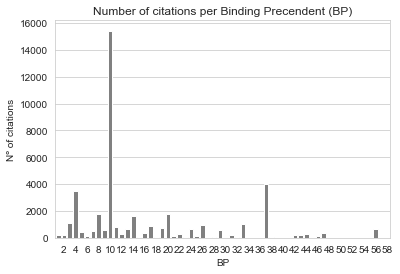
\includegraphics[width=0.8\linewidth]{bp_citations.png}
        \end{figure}
    \end{frame}

    \begin{frame}
        \frametitle{Exploratory data analysis}
        \begin{figure}
            \centering
            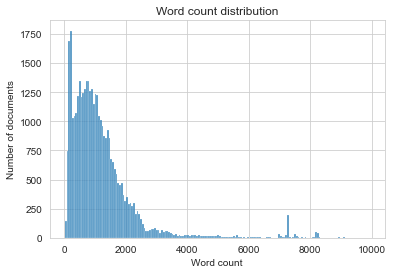
\includegraphics[width=0.8\linewidth]{word_count.png}
        \end{figure}
    \end{frame}

    \begin{frame}
        \frametitle{Exploratory data analysis}
        \begin{figure}
            \centering
            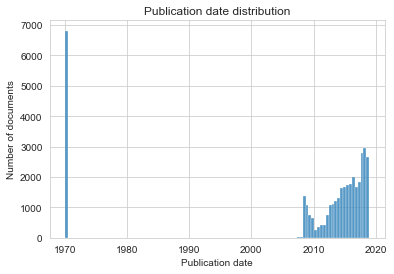
\includegraphics[width=0.8\linewidth]{dates.png}
        \end{figure}
    \end{frame}

    \begin{frame}
        \frametitle{Document embedding}
        Before texts can be fed into machine learning models, they need to become numbers, usually vectors. These vectors are called text embeddings, and, in the case of long texts, document embeddings. \pause
        \begin{itemize}
            \item TF-IDF: it counts the frequency of this word relative to this document (term frequency - TF). This count is ``normalized'' by the rarity of the word in the entire set of documents (inverse document frequency - IDF); \pause
            \item Dimensionality reduction: truncated singular value decomposition.
        \end{itemize}
    \end{frame}

    \begin{frame}
        \frametitle{Machine learning models}
        We experiment with many models.
        \begin{itemize}
            \item Latent Dirichlet allocation;
            \item Truncated SVD dimentionality reduction;
            \item K-nearest neighbors;
            \item Linear regression;
            \item Logistic regression;
            \item Linear discriminant analysis;
            \item Random forest;
            \item Support vector machines.
        \end{itemize}
    \end{frame}

    \begin{frame}
        \frametitle{Sample dataset}
        Because the original dataset is very unbalanced among the Binding Precedent citations, we need to create a sample dataset that will be used in our analysis. We consider: \pause
        \begin{itemize}
            \item each document cites only one BP, to avoid confusion;\pause
            \item documents that share the same raw texts are removed, to avoid overfitting;\pause
            \item we only work with the five most cited BPs, for simplicity and also data limitation;\pause
            \item the dataset is balanced among the classes, \ie, each class has the same number of documents.\pause
        \end{itemize}
        In the end, we work with 1401 documents of BPs 10, 37, 4, 20, and 14, totalizing 7005 documents.
    \end{frame}

    \begin{frame}
        \frametitle{Latent Dirichlet allocation}
        Choosing five topics, we have: \pause
        \begin{figure}
            \centering
            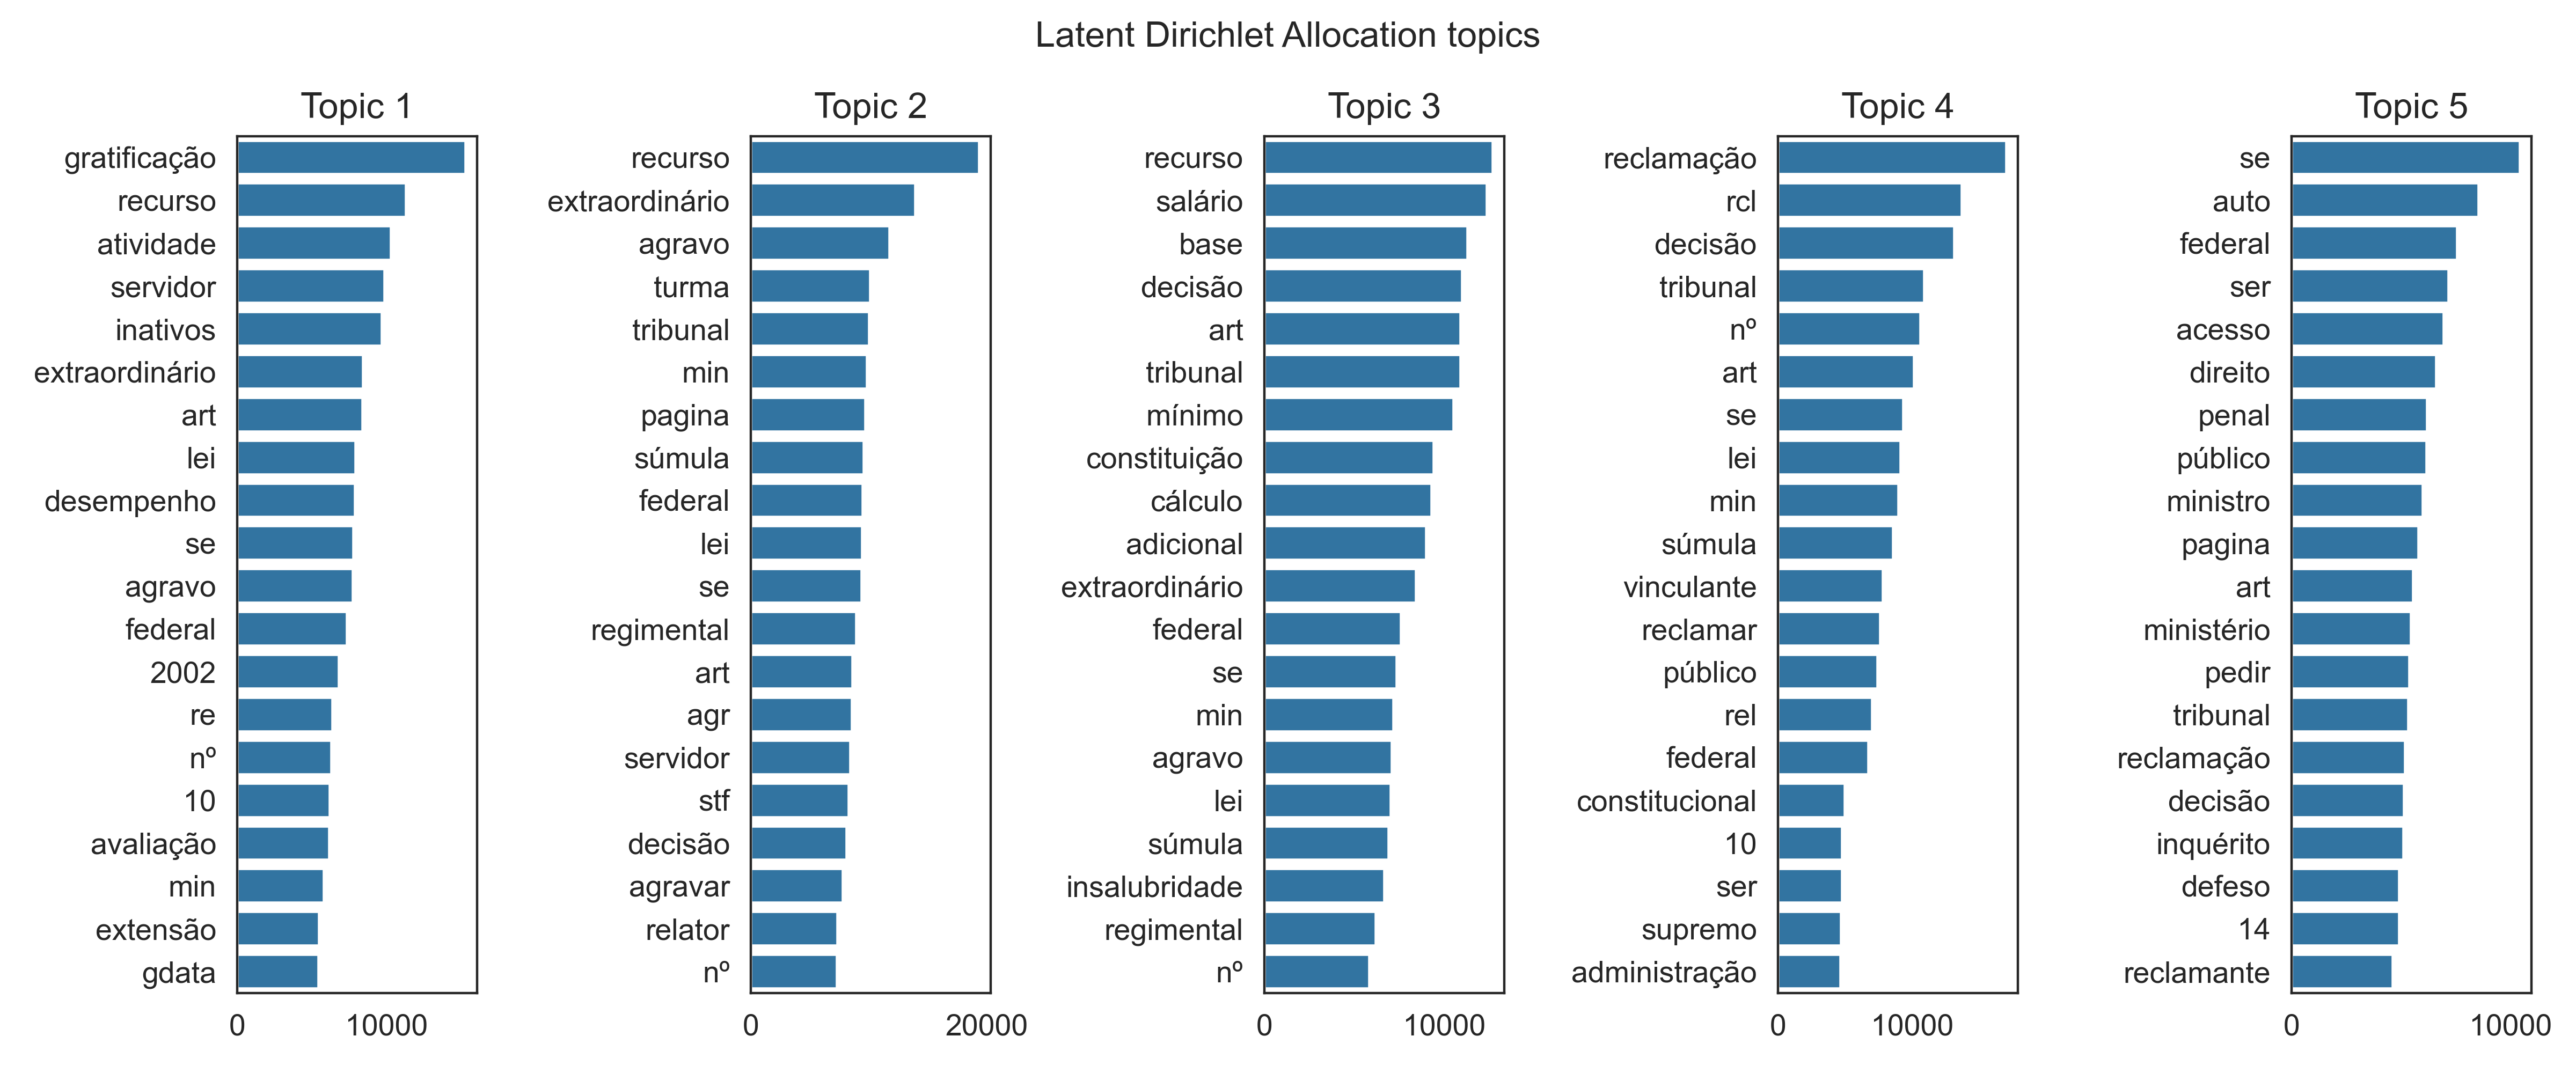
\includegraphics[width=\linewidth]{lda_topics.png}
        \end{figure}
    \end{frame}

    \begin{frame}
        \frametitle{Latent Dirichlet allocation}
        From the barplot, we can see the following topics associated with the following BPs, justified by the following words:
        \begin{itemize}
            \item topic 1 \& BP 20: gratificação, inativos, atividade, desempenho, avaliação, gdata;
            \item topic 3 \& BP 4: salário, base, decisão, mínimo, constituição, cálculo;
            \item topic 4 \& BP 10: decisão, tribunal, constitucional, 10;
            \item topic 5 \& BP 14: acesso, direito, penal, inquérito, defeso, 14.
        \end{itemize}
        \pause
        Using this topic to BP assignment presented before, we get an accuracy of 0.76. That is, this topic modeling predicts the cited precedent correctly in 76\% of documents. We would expect 0.2 if it were a random assignment.
    \end{frame}

    \begin{frame}
        \frametitle{Truncated SVD dimensionality reduction}
        \begin{figure}
            \centering
            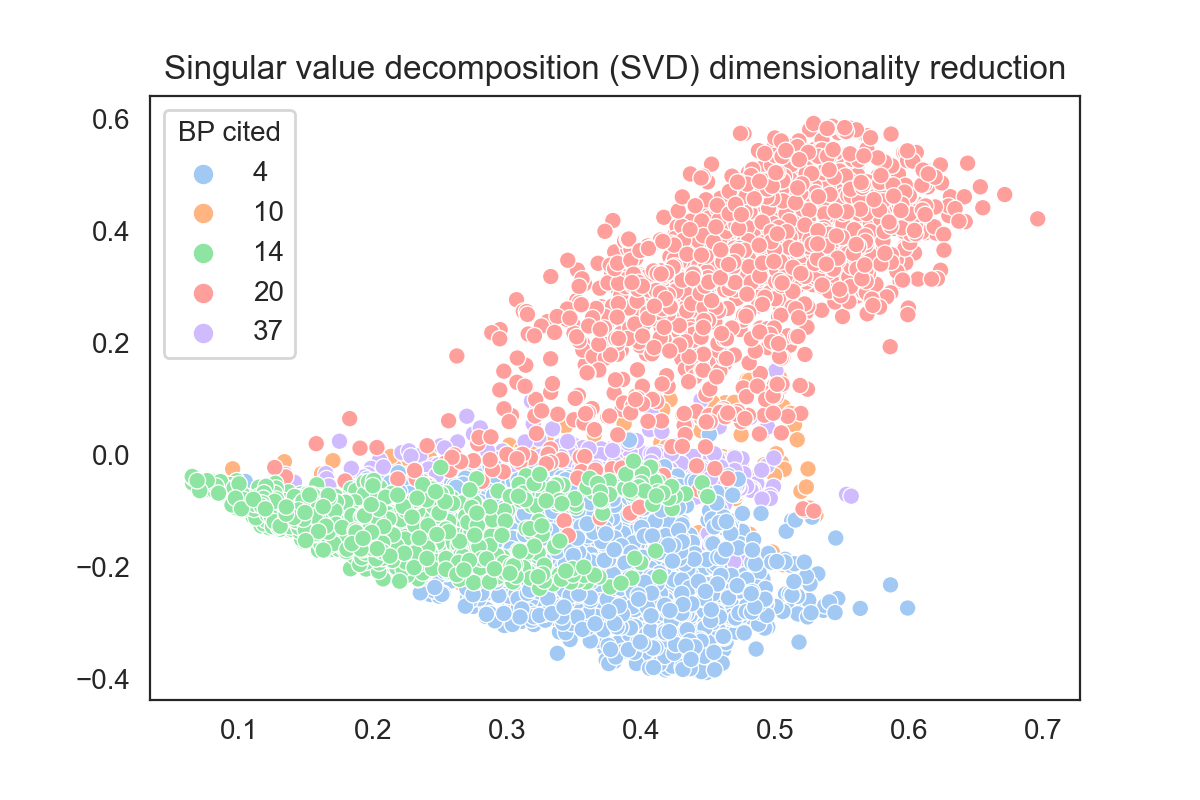
\includegraphics[width=0.8\linewidth]{svd_1.png}
        \end{figure}
    \end{frame}

    \begin{frame}
        \frametitle{Truncated SVD dimensionality reduction}
        \begin{figure}
                \centering
                \subfloat[\centering ]{{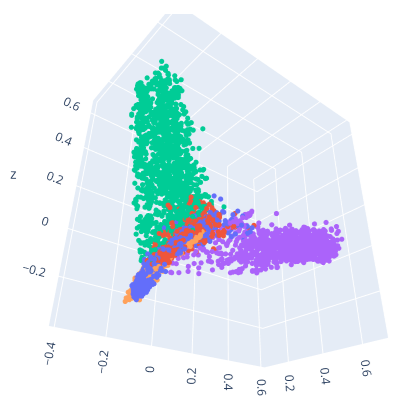
\includegraphics[width=0.4\linewidth]{svd_2.png} }}
                \qquad
                \subfloat[\centering ]{{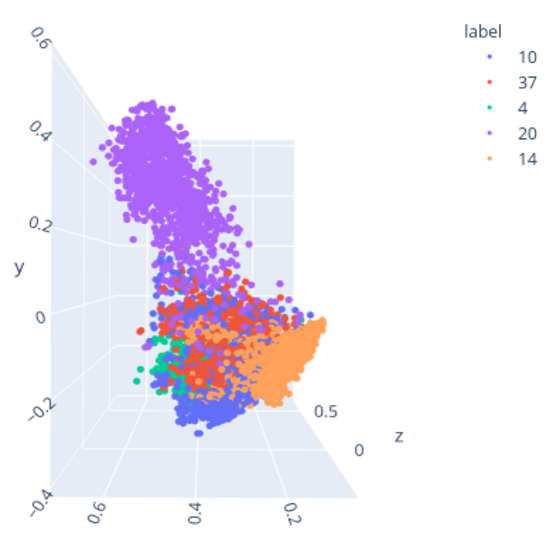
\includegraphics[width=0.4\linewidth]{svd_3.png} }}
        \end{figure}
    \end{frame}

    \begin{frame}
        \frametitle{Support vector machine}
        \begin{table}[H]
            \centering
            \caption{Support vector machine test metrics.}
            \label{tab:svm}
            \begin{tabular}{c|cc|c}
            BP & Precision & Recall & Accuracy              \\ \hline
            4  & 0.99      & 0.97   & \multirow{5}{*}{0.97} \\
            10 & 0.95      & 0.97   &                       \\
            14 & 0.98      & 0.99   &                       \\
            20 & 0.98      & 0.97   &                       \\
            37 & 0.96      & 0.96   &                      
            \end{tabular}
        \end{table}
    \end{frame}

    \begin{frame}
        \frametitle{Support vector machine}
        \begin{figure}
            \centering
            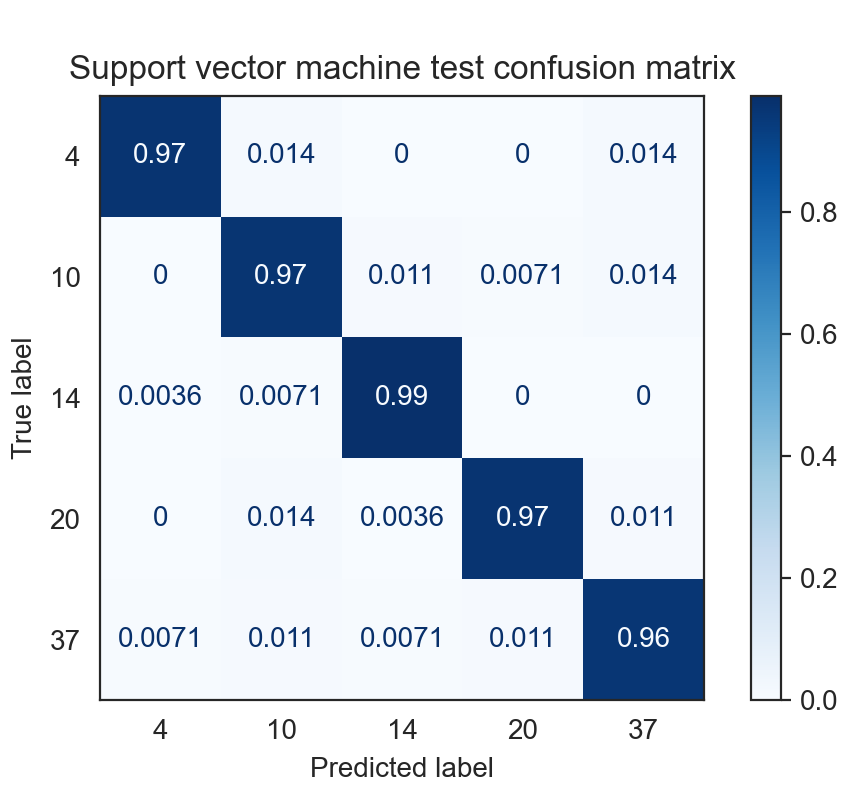
\includegraphics[width=0.6\linewidth]{svm.png}
        \end{figure}
    \end{frame}

    \begin{frame}
        \frametitle{Further discussion}
        \begin{figure}
            \begin{flushleft}
                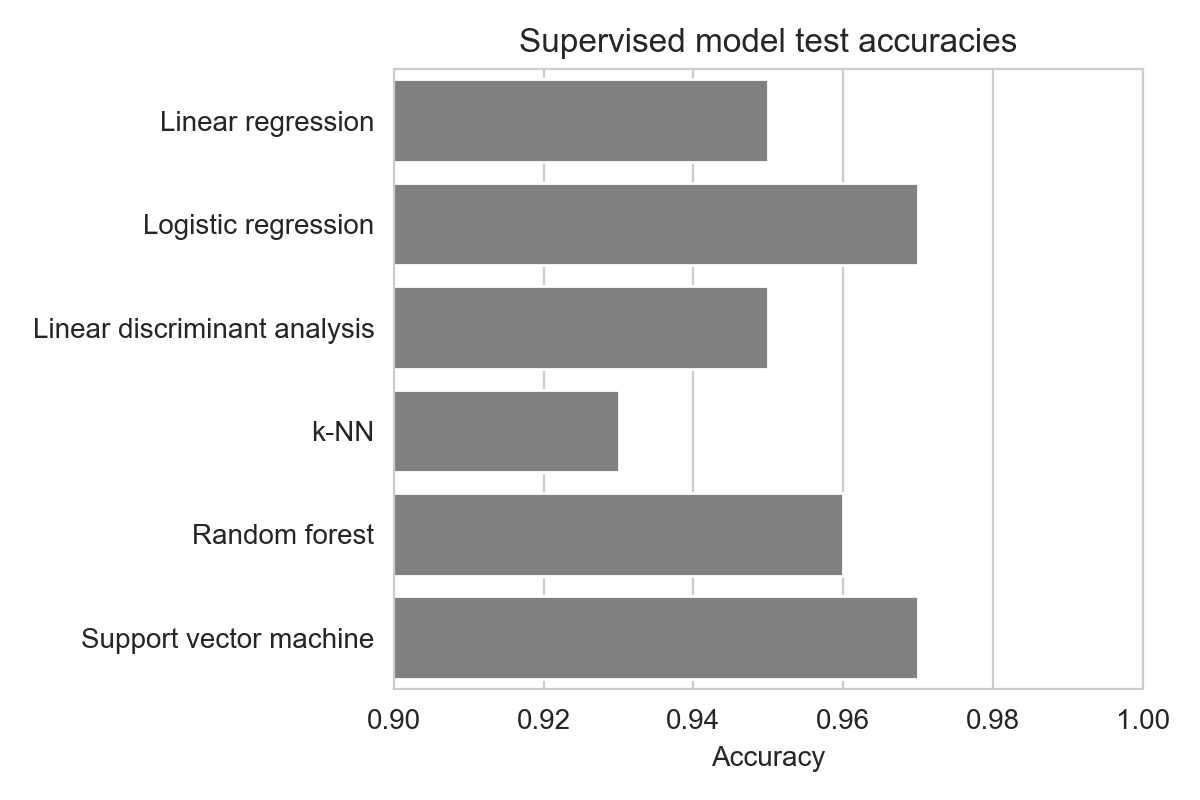
\includegraphics[width=0.8\linewidth]{accuracies.png}
            \end{flushleft}
        \end{figure}
    \end{frame}

    \begin{frame}
        \frametitle{Further discussion}

        \begin{itemize}
            \item It is clear from the experiments that our dataset is separable; \pause
            \item Even more, the data seems to be \textbf{linearly separable} (indicated by linear regression, logistic regression, and linear discriminant analysis); \pause
            \item The documents, in very high dimensional space, are closer if they cite the same precedent (truncated SVD dimensionality reduction and k-NN); \pause
            \item The LDA topics extracted words and the subject of the cited precedents. With five BPs and five topics, each topic could be associated with a BP, with high accuracy.
        \end{itemize}
    \end{frame}

    \begin{frame}
        \begin{center}
        {\Huge Thank you!}
        \bigskip

        Lucas Emanuel Resck Domingues \\
        \textit{School of Applied Mathematics} \\
        \textit{Getulio Vargas Foundation} \\
        \textit{lucas.domingues@fgv.edu.br} \\
        \textit{github.com/lucasresck/machine-learning/}
        \end{center}
    \end{frame}

    \nocite{*}
    \bibliographystyle{alpha}
    \bibliography{sample}

\end{document}